
\subsection{稳态转换潜在驱动期识别}

根据气候湿润与人类活动两类驱动因素的组合,本章研究将黄河在历史时期的驱动因素变化过程分为七个时期(表\ref{tab:ch3:periods_division})。
在公元400年之前,由于所有原始数据的可信度均较低,因此本研究不再后续分析中讨论(图\ref{fig:ch3:drivers}~A)。
过去的2000年间,研究区的大多数时期均偏干燥,记录了223次极旱年和182个洪泛年,因此强烈湿润的气候驱动时段较少。
结合湿润指数,本章研究为黄河流域在过去两千年中识别出三个潜在的气候驱动期(CDPs),其中有两个在数据可靠的时期,分别开始于公元900AD和1700AD(图\ref{fig:ch3:drivers}~B)。
另一方面,在公元900年之前几乎没有人类活动驱动的迹象(图\ref{fig:ch3:drivers}~C)。
虽然900AD\textendash{}1000AD间农业区域向北扩大可能指示人类活动的增强,但由于缺乏可靠的人口增长证据,且气候暖湿化也会引起农区扩张,所以此时段在本研究中不被认为是一个确定的人类活动驱动时段(HDP)。
而在这之后的1450年至1650年以及1900年后,随着人口显著增加和农牧交错带向北移动,本研究将这两个时段认为是需要分析的人类活动驱动时期(HDPs)。

% Table generated by Excel2LaTeX from sheet '历史时期特征划分'
\begin{table}[htbp]
    \centering
    \caption{基于驱动因素的历史时段划分及其特点}
      \begin{tabularx}{\textwidth}{LLL}
      \toprule
      时间跨度  & 时段划分  & 主要特征 \\
      \midrule
      200BC-400AD & 数据不可信时段 & 各数据集在此时期的可信度均偏低 \\
      400-900AD & CDP1前期 & 没有明显的驱动因素 \\
      900-1100AD & CDP1时期 & 气候驱动与低水平的人类活动驱动时期 \\
      1100-1350AD & CDP1后期 & 没有明显的驱动因素 \\
      1350-1700AD & CDP2前期 & 人类活动驱动时期 \\
      1700-1900AD & CDP2时期 & 气候驱动与人类活动共同驱动时期 \\
      1900-2000AD & HDP2时期 & 人口迅速增长的人类活动强烈驱动期 \\
      \bottomrule
      \end{tabularx}%
    \label{tab:ch3:periods_division}%
\end{table}%
  

% \begin{rotate
\begin{figure}[!ht]
    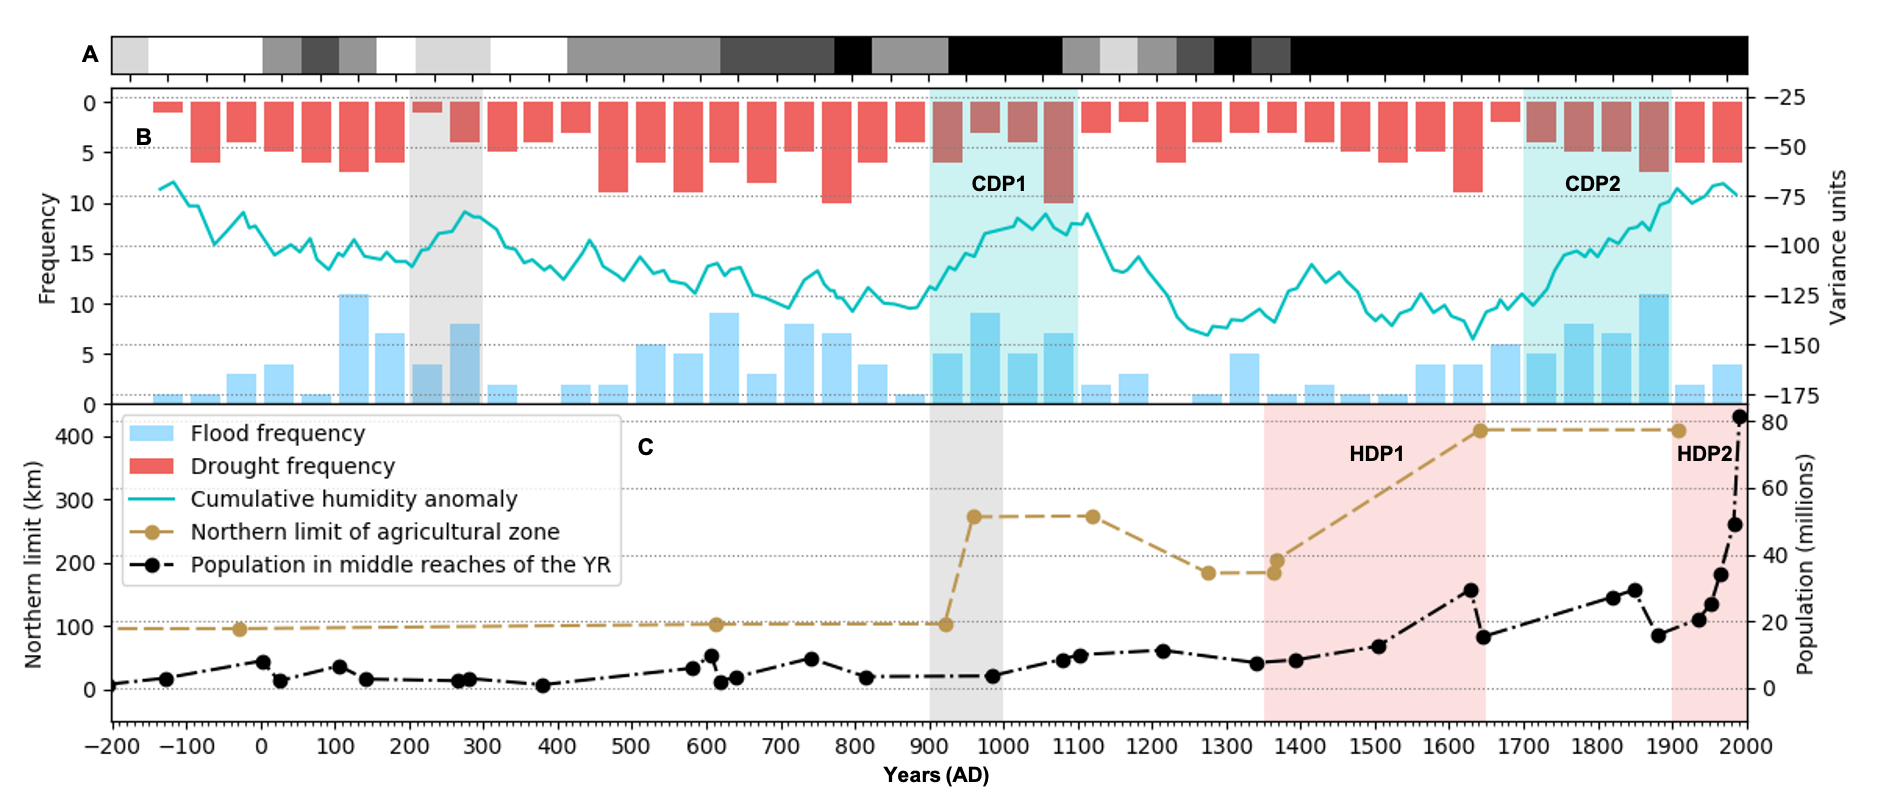
\includegraphics[width=\textwidth]{img/ch3/ch3_drivers.png}
    \caption[黄河流域历史时期稳态转换的驱动力变化]{黄河流域历史时期稳态转换的驱动力变化。
    \textbf{A} 原始数据有五级综合置信度($0 \textendash{} 1$),分别从极低置信度(白色)到极高置信度(黑色);
    \textbf{B} 气候驱动时期:用极端气候频率(干旱或洪水)以及累积湿润度距平共同确定的两个明显的气候驱动时段(CDPs),由蓝色阴影表示;
    \textbf{C} 人类活动驱动时期:根据黄河中游人口增长和农牧交错带北界的移动情况确定的人类活动驱动时段(HDPs),由红色阴影表示$^*$。}
    \footnotesize
    * 灰色阴影的部分表示农牧交错带北极界移动,但因缺乏可靠的人口增长证据且气候湿润也会引起农区扩张,所以不认为是一个人类活动驱动时段(HDP)。\label{fig:ch3:drivers}
\end{figure}

\subsection{稳态转换的影响因素变化}

根据上述时段划分,自CDP1开始(图\ref{fig:ch3:impacts}~CDP1),黄河的决溢现象更加频繁,三门峡通航也变得更容易,同时下游两个样品的沉积速率也超过了$4cm/yr$,显示出湿润气候驱动力的影响。
然而在CDP1之后,尽管没有通过沉积样品评估泥沙量,但洪泛频率的降低与重新变差的航运情况表明,黄河的情况重新回到了CDP1之前的时期。
最后,在进入第一个明显的人类驱动时期(HDP1)时,更多的沉积样品表现出下游泥沙沉积速率明显上升的趋势(图\ref{fig:ch3:impacts}~HDP1\textendash{}HDP2),并伴随更频繁的洪泛和持续糟糕的航运水平。


根据数据的可信度,图\ref{fig:ch3:impacts}提供了两个气候驱动期(CDP)前、中、后期的情况对比。
首先,直接反映输沙量的沉积率指标在HDP1之后的可信度一直较低,直到第二个人类驱动时期(HDP2)结束后才有较为可靠的增加证据(图\ref{fig:ch3:impacts}~E和F)。
其次,尽管这两个湿润的气候驱动时期都让洪泛频率明显增加(图\ref{fig:ch3:impacts}~D和E),但只有在第一个气候驱动期(CDP1)时航运更加便利,而在第二个气候驱动期结束后(CDP2,恰好也是人类活动强烈驱动期 HDP2)反而航运更加困难了。
综上所述,虽然气候存在周期性,但第一个强烈的气候驱动期(CDP1,900AD \textendash{} 1100AD)和第二个气候驱动期(CDP2,1700AD \textendash{} 1900AD)已呈现出不同的流域系统过程。

\begin{figure}[!ht] % use float package if you want it here
    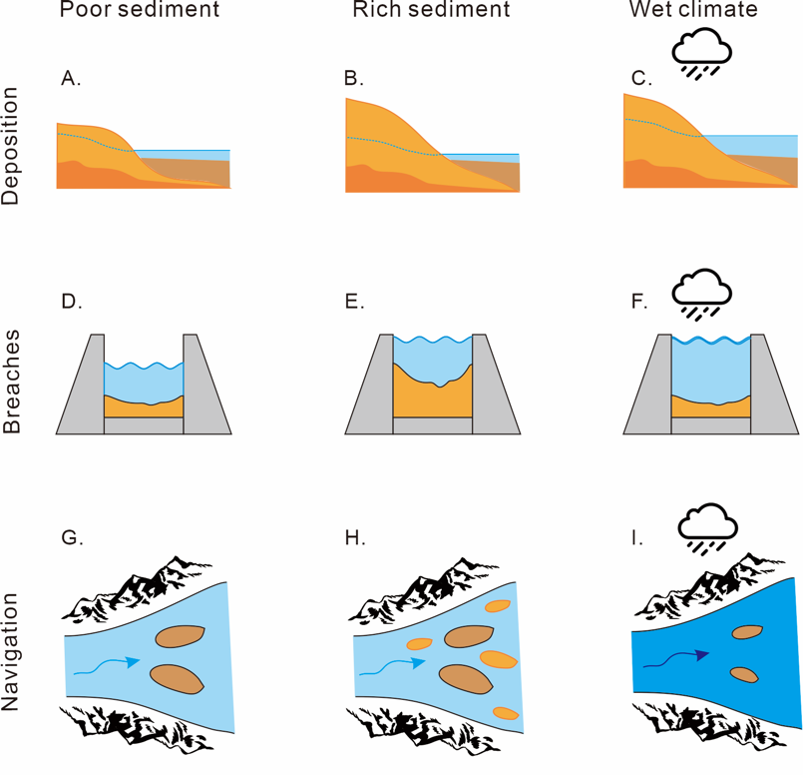
\includegraphics[width=\textwidth]{img/ch3/ch3_impacts.png}
    \caption[历史时期各时段的影响因素与信度变化]{历史时期各时段的影响因素与信度变化。每个时段内(气候驱动时段CDP,或人类活动驱动时段HDP),沉积(黄色)、洪泛(蓝色)、航运(红色)三个典型受影响因素的特征等级与可信度等级(见\ref{sec:ch3:approach}\nameref{sec:ch3:approach})。
    在每个半圆内,扇形的半径表明影响因素的强度等级,弧长表示其数据可信度。由于航运和洪泛滥同水量变化是相反的,本章研究将它们放在扇形的不同象限,从而使扇形左右两个方向分别代表更少的水量与更多的水量。简而言之,某个颜色的扇形面积更大,就有越大的把握说明该时段内的此影响因素强度。$A$ \textendash{} $F$分别代表被两次气候驱动期CDP所分割的不同时段: (A) 400AD\textendash{}900AD (B) 900AD \textendash{} 1100AD (C) 1100AD\textendash{}1350AD (D) 1350AD\textendash{}1700AD (E) 1700AD \textendash{} 1900AD 和 (F) 1900AD\textendash{}2000AD。}\label{fig:ch3:impacts}
\end{figure}
